\documentclass[openany]{memoir}

\usepackage[utf8]{inputenc}
\usepackage{fullpage}
\usepackage{graphicx}
\usepackage{hyperref}
\usepackage{tcolorbox}
\usepackage{pifont}
\usepackage{float}
\usepackage{listings}
\usepackage{svg}
\usepackage[intlimits]{mathtools} 

\lstset{
resetmargins=true,
frame=single,
breaklines=true, 
breakatwhitespace=true,
backgroundcolor=\color[RGB]{240,240,240}
}

\chapterstyle{ell}

\setcounter{secnumdepth}{3}
\setcounter{tocdepth}{2}

\title{TargetOptimizer 2.0 User Manual}
\date{\today}

\begin{document}

\maketitle

\tableofcontents*

\setlength{\parindent}{0pt}

\chapter{Introduction}

This chapter will give a short introduction to getting TargetOptimizer 2.0 up and running and what to use it for. For more details please refer to \autoref{chap:overview} and \autoref{chap:synthesis}.

\section{Purpose}
TargetOptimizer 2.0 (TO2) is a free and open-source PC software to estimate pitch targets parameters of the Target Approximation Model (TAM) from the $f_{0}$-contour of spoken utterances.\\
TO2 allows not only the reproduction of natural pitch contours with a small error but also yields more ``natural" pitch targets in the sense of TAM, which can be used as an intonation model for text-to-speech synthesis. This simplifies the copy-synthesis of natural utterances using articulatory speech synthesizer.

\section{Downloads}
TO2 is distributed as free and open source software under the GNU General Public License (GPL). It is written in C++ and developed for both Windows and Linux platform.
The software is free of charge and available at \ding{43} \href{https://www.vocaltractlab.de/index.php?page=targetoptimizer-download}{VocalTractLab-website} or as a clone from \ding{43} \href{https://github.com/TUD-STKS/TargetOptimizer}{git repository}. Binaries for Windows OS and C++ sources of the software are included, together with some example files.

\section{Installation}
To install the software in Windows, simply unzip the downloaded file into a folder of your choice. The archive contains an executable (.exe) to start the Graphical User Interface (GUI), some dynamic link libraries (*.dll) and the example files.


\section{Execution}
The software can be executed as an application including a GUI or as a command line tool to support batch processing. To execute the software on Windows, simply run the application file ``TargetOptimizer.exe" to start the GUI, or type ``TargetOptimizer.exe -h" on the command line options for instructions. On Linux you have to build the project by yourself. For more information see \autoref{sec:build}.\\
In addition, you can use the TargetOptimizer functions in the API within your own software. Some Matlab and Python code examples demonstrate how to use it. In \autoref{chap:synthesis} it is shown how to use TO2 as a part of an articulatory synthesis pipeline.

\section{Build instructions}\label{sec:build}
Both the GUI and API version can be further developed and compiled by yourself. The GUI version contains a project file for Visual Studio 2019 in Windows, but it can also be compiled under Linux or Mac. The only external library required is the cross-platform GUI library \ding{43}  \href{www.wxwidgets.org}{wxWidgets}.\\ 
The following indicates how to compile the source code of the software:
\begin{itemize}
	\item Windows: \\
	Simply open the solution ``TargetOptimizer.sln" and build in dependency of desired use case:
	\begin{itemize}
		\item ``Release" - for command line tool				
		\item ``wxWidgets\_Release" - for GUI version using wxWidgets
		\item ``wxWidgets\_VCPKG\_Release" - for GUI version using \ding{43}  \href{https://www.wxwidgets.org/blog/2019/01/wxwidgets-and-vcpkg/}{VCPKG and wxWidgets} 
	\end{itemize}
	Note: ``TargetOptimizer.exe" can always be found in the sub-folder ``x64" in dependency on your chosen build configuration.
	\item Linux: \\
	Navigate inside the source folder and run one of the following commands:
	\begin{itemize}
		\item For the command-line-only version:
	\end{itemize}
	\begin{lstlisting}[mathescape=true]
	g++ -std=c++14 -O3 -I.. ../dlib/all/source.cpp -fopenmp -lpthread -lX11 $^\ast$.cpp -o TargetOptimizer
	\end{lstlisting}
	\begin{itemize}
	    \item For the GUI version (requires wxWidgets):
	\end{itemize}
	\begin{lstlisting}[mathescape=true]
	g++ -std=c++17 -O3 -D USE_WXWIDGETS -I.. ../dlib/all/source.cpp -fopenmp -fpermissive -lpthread -lX11 $^\ast$.cpp `wx-config --cxxflags --libs std` -o TargetOptimizer -w -lstdc++fs
	\end{lstlisting}
\end{itemize}

\section{Use and license information}
As stated before, the offered software is free and open-source under the GNU General Public License.\\ 
You can refer the software by citing the most recent paper

\begin{itemize}
\item[\ding{71}]
Paul Konstantin Krug, Simon Stone, Alexander Wilbrandt, Peter Birkholz. TargetOptimizer 2.0: Enhanced estimation of articulatory targets. \cite{TO2}
\end{itemize}

This paper also includes more specific information on the changes between the TargetOptimizer 1.0 and 2.0.\\
Note that the software comes with no warranty of any kind. There was no extensive test of the software, but the parts of the programs made available are considered relatively stable. The whole software is under continual development and may undergo substantial changes in future versions. Please feel free to report any bugs by using the \ding{41} \href{https://github.com/TUD-STKS/TargetOptimizer/issues/new}{issue tracker of the git repository}.
\chapter{Overview}\label{chap:overview}
In the following sections, the computational models underlying TO2 will be explained. The GUI and the usage of TO2 as commandline tool will be described in detail as well.\\
The main features of TO2 are:
\begin{itemize}
\item The $f_{0}$ contour in the voiceless parts of the original utterance is not interpolated before the target estimation compared to PENTAtrainer1 \cite{TAM1} and PENTAtrainer2 \cite{TAM2} because it is not guaranteed that the interpolated sections support the optimal reproduction of $f_{0}$ in the truly voiced sections.
\item The targets for all syllables of the utterance are jointly optimized, instead of one syllable after the other.
\item The regularization is used to prefer natural or plausible pitch targets, since different combinations of TAM parameters can generate almost identical $f_{0}$ contours.
\item The TAM adopts 5th-order systems instead of 3rd-order systems, as they allow a more accurate modeling of pitch contours.
\item The position of the target boundary positions are adjustable in the optimization process to obtain a better pitch contour in terms of minimized RMSE. The target boundaries can be as well initialized uniformly distributed across an utterance to use them as start parameters.
\item The hyper-parameters of the optimization algorithm can be adjusted by the user, e.g., the iteration depth and the usage of early stopping.
\end{itemize}

\section{Computational models}
TO2 uses various models, including target approximation model, the models for estimation of target boundaries and early stopping. This section provides the most important information on those models from the papers \cite{TO1} and \cite{TO2}, which you should consider reading if you wish to understand them in-depth.

\subsection{Target Approximation Model}
The Target Approximation Model (TAM) \cite{TAM1, TAM2} is a well-known intonation model that does not only allow the generation of very natural pitch contours, but can also be used to produce realistic trajectories of articulators, which is especially useful for articulatory speech synthesis \cite{VTL}. To create highly realistic pitch or articulatory trajectories, natural acoustic or articulatory speech data can be used as a reference.\\ 
The TAM assumes one pitch target for each syllable of an utterance. According to \cite{TO1}, the target $x(t)$ is defined within the interval of a syllable as the linear function $x(t)=mt+b$, where $m$ (in st/s) and $b$ (in st) denote the slope and height of the target, respectively. The time $t$ is defined relative to the onset of the syllable for the interval $[0,d]$, where $d$ is the syllable duration. The $f_{0}$ (in st) within the syllable is the response of a critically-damped low-pass filter of the order $N$ (i.e., the concatenation of $N$ identical first-order low-pass filters) with the time constant $\tau$. At the beginning of the first syllable of an utterance, $f_{0}$ is given as an onset value $\phi$ and the derivatives of $f_{0}$ are set to zero. We used the time constant $\tau$ to characterize the linear system.\\
For the estimation of pitch targets based on TAM, we assume that the pitch contour is given in terms of samples $f_{0}(k\Delta t)$ in the voiced parts of the corresponding utterance, where $\Delta t$ is the sampling interval (typically $10\,ms$) and $k$ is the sampling index. We also assume that the syllable boundaries are given, and hence the target duration. The unknown parameters of the TAM are slope $m_{s}$, offset $b_{s}$, and time constant $\tau _{s}$ of every syllable (i.e., target) $s$. These parameters can be summarized in vectors $\mathbf{p}_{s}=(b_{s},m_{s},\tau_{s})^{\mathrm{T}}$, where $s=1,2,\dots,S$ and $S$ is the number of syllables. The initial $f_{0}$ value $\phi$ of the TAM is set to the first $f_{0}$ sample of the utterance. In contrast to the previous approaches implemented in \cite{TAM2}, we propose the joint estimation of all TAM parameters by regularized optimization, which has a better chance to find an optimal solution for the whole utterance. In addition, regularization helps to obtain solutions that are not only optimal in a mathematical sense but also physiologically most plausible. The proposed objective function to be minimized is
\begin{equation}\label{min}
\mathit{g}(\mathbf{p}_{1}\dots \mathbf{p}_{S})=\left \| f_{0}(k\Delta t)-\hat{f_{0}}(k\Delta t,\mathbf{p}_{1}\dots \mathbf{p}_{S}) \right \|_{2}^{2}+\lambda \sum_{s=1}^{S}(\mathbf{p}_{s}-\mathbf{\bar{p}})^{\mathrm{T}}W(\mathbf{p}_{s}-\mathbf{\bar{p}})
\end{equation}
The first term on the right-hand side of Eq.\ref{min} is the squared Euclidean distance between the original $f_{0}$ samples in the voiced parts of the utterance and the corresponding values $f_{0}$ generated by the TAM. The second term is the regularization term that penalizes parameter values based on their deviation from the preferred values $\mathbf{\bar{p}}=(\bar{m},\bar{b},\bar{\tau})^\mathrm{T}$. The degrees of penalization for the different TAM parameters are adjusted by the elements of the weight matrix $W=\mathrm{diag}(w_{m},w_{b},w_{\tau})$, and $\lambda$ determines the overall degree of regularization. The weights were empirically adjusted to $w_{m}=1\: s^{2}/st^{2}$, $w_{b}=0.6\: st^{-2}$, and $w_{\tau}=0.2\: s^{2}$. We furthermore set $\bar{m}=0$ (static targets are preferred) and $\bar{\tau}=12.5\,ms$ (this is considered as the ``typical" time constant). $\bar{b}$ was set to the average pitch of the corresponding natural utterance. The bounds for $\tau$ were adopted from \cite{TAM2}, and the bounds for $b$ were adjusted to cover a frequency range of $76-767\,Hz$.\\
In principle, the optimization problem above can be solved using any method for bound-constrained optimization that requires only the availability of an objective function but no derivative information \cite{DFO}. Here we used the algorithm Bounded Optimization by Quadratic Approximation (BOBYQA) \cite{BBQ}, which is available as a C++ implementation in the modern open-source software toolkit dlib \cite{Dlib}. Like most optimization methods for non-convex problems, BOBYQA cannot guarantee to find the global minimum of the objective function. Accordingly, the method should be run multiple times with different random initial parameter values (within the respective bounds), and the best solution should be selected. Here we used $5S+10$ random initialization per optimization, as the complexity of the problem increases with the number of syllables $S$.

\subsection{Estimation of target boundaries}
Within the TO2 framework, the parameter set is extended by a fourth parameter $\delta_{B}$ referred to as boundary delta. In contrast to the other parameters that are optimized as absolute values, the boundary delta is a relative value between -1 and 1. At each step of the BOBYQA optimization procedure, the onset of each target is changed relatively to the initial position of the corresponding boundary. Considering a number of $N$ articulatory targets, the initial target onset positions are given by $T_{n}$ (in ms), where $n=1,\dots N$. According to \cite{TO2}, the boundaries are shifted with respect to the duration of the preceding (succeeding) target if the boundary delta is negative (positive). Therefore, target boundaries can not shift beyond the initial onset boundaries of adjacent targets. However, shifted targets might move beyond a preceding shifted target. If this happens, boundaries are reordered to be monotonically increasing in time, so that the individual targets are always well defined and never overlap. Since there is no preceding target in the case of $n=1$, the maximum negative time shift of the first boundary was defined as $-100\,ms$. Even though there should be no trajectory data before the first initial boundary, a shift of the first boundary towards an earlier time instant can be beneficial due to the initialization and the impulse response of the TAM filter. On the other hand, if the time shift of the first boundary is positive, it might move past the first data point. To prevent this, the first boundary is set to the time of the first data point in such a case. The offset of the last target $N$ (boundary number $N+1$) does not get optimized. It is always set equal to the time point of the last data point, since the region beyond the last data point has no influence on the fit.\\
In addition, the maximum possible boundary shift $[-\delta_{B,max},+\delta_{B,max}]$ is controlled by user. If $\delta_{B,max}<1$, the boundary optimization is limited to a respectively smaller region around the initial boundaries and setting it to zero restores the TO1 behavior (no boundary optimization). If boundary optimization is activated and $\delta_{B,max}=1$, the optimal position of all target boundaries in principle can be estimated from any given initial configuration of boundaries. Therefore, an initialization by prior syllable annotation is no longer a necessary requirement as it was in TO1. Instead, the TO2 provides the possibility to initialize the boundaries at evenly spaced positions between the first and last data point.

\subsection{Early stopping}
Since the BOBYQA algorithm does not necessarily find the global minimum of the objective function in a single run, the optimization procedure must be executed multiple times, each time initialized with a different set of parameters drawn at random from the defined search space. In the following, such multiple runs are referred to as random iterations. The random iterations are independent from each other and the run that minimizes the objective function is selected as the optimization result. The number of random iterations is a tunable parameter in TO2 that can be adjusted by user. This is important because the boundary optimization added another dimension to the search space and the computational complexity of the problem increased. Therefore, runs with boundary optimization require a lot more random iterations to converge to the optimum, compared to runs without boundary optimization. On the other hand, additional random iterations become unnecessary once the optimum is found. In order to reduce the computational cost, a method referred to as early stopping has been developed to terminate the search prematurely as soon as a certain convergence criterion is met. Through the procedure of early stopping shown in \cite{TO2}, a temporary minimum of the TO objective function of each respective random iteration must be smaller than the current minimum (the global minimum across the multiple iterations) minus a percentage of the current minimum (determined by the hyper-parameter $\epsilon$ that can be set by user), in order to be counted as the new (temporary) global minimum. If the global minimum is updated, a convergence counter (that is increased by one after every iteration) is reset to zero. Once the convergence counter reaches a certain value referred to as patience, the search is terminated. The patience is another hyper-parameter that can be adjusted by user.\\
In addition, the BOBYQA optimization algorithm has two important hyper-parameters: the maximum number of cost evaluations $N_{f}^{max}$ (the objective function evaluations per single random iteration), and the final trust region radius $\rho_{E}$. In TO2, both parameters can be adjusted by user. Nevertheless, since these parameters can have a huge impact on the performance and the computational costs, good default values were estimated via a grid search. Since this tuning of hyper-parameters was time-consuming from a computational point of view, it was not performed on the whole speech corpus, but only on a small subset of 8 utterances. In this subset, all syllable numbers were represented once. The parameter $N_{f}^{max}$ was modified in ten equal steps from $10^5$ to $10^6$ and $\rho_{E}$ was varied in four steps by four orders of magnitude from $10^{-6}$ to $10^{-3}$. Each combination of utterances and parameters was evaluated, giving a total of 320 TO2 runs with boundary optimization. The number of random iterations per run was set to 1000 and early stopping was disabled.

\section{ Graphical User Interface (GUI)}
As mentioned above, the TO2 can be used via a GUI. Fig.\ref{GUI} shows the layout of this GUI. From top to bottom, it consists of a title bar, a menu bar, the main window region, and the control panel. 
\begin{figure}[H]
\centering
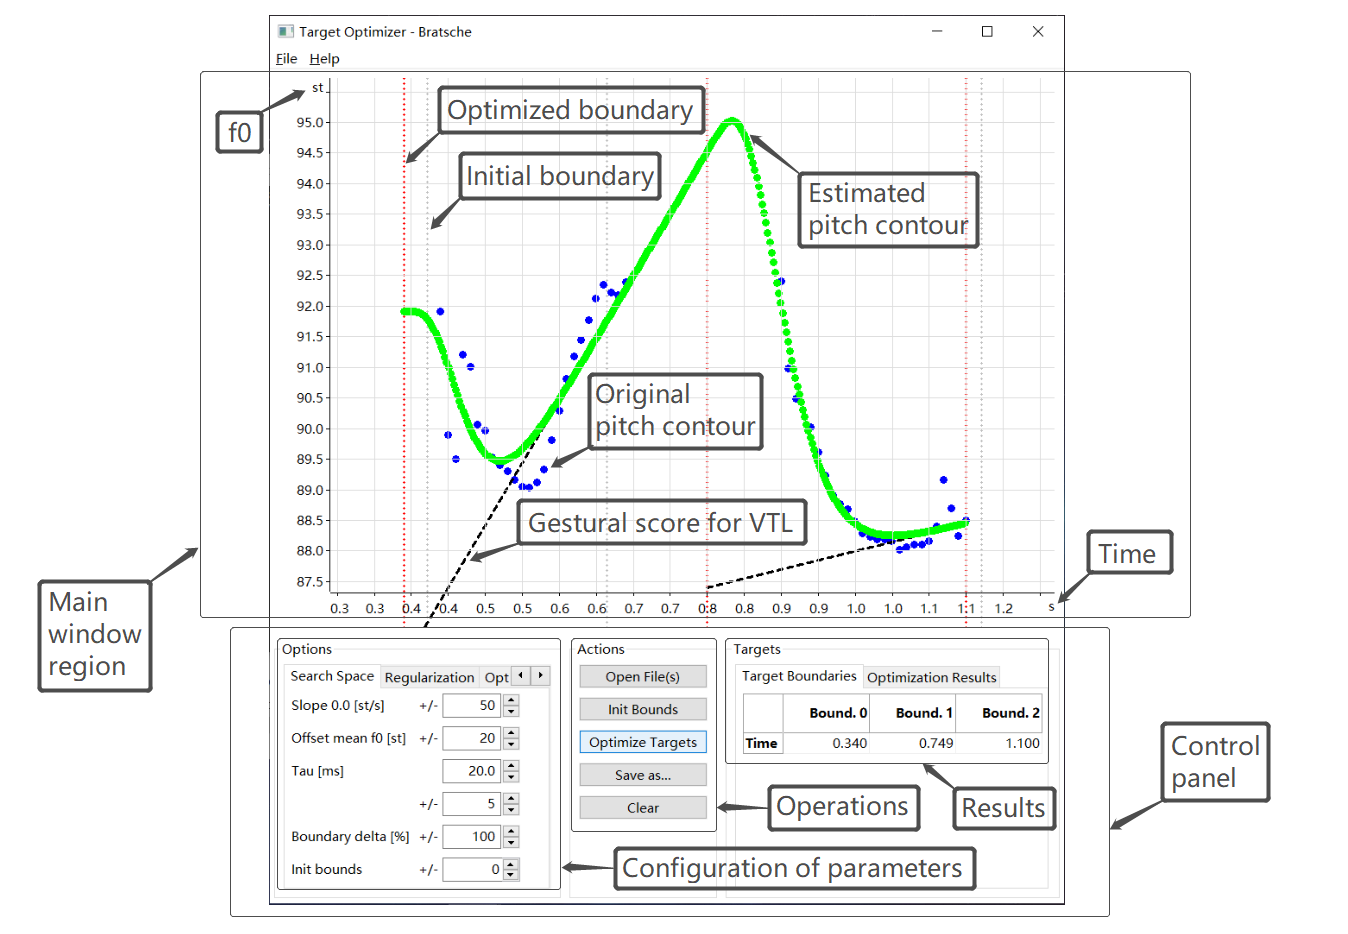
\includegraphics[width=\textwidth]{images/GUI.png}
\caption{GUI of the TargetOptimizer 2.0}
\label{GUI}
\end{figure}

\subsection*{Menu bar} 
The menu bar has two menus ``File" and ``Help".\\ 
The ``File" menu includes six items: ``Open File(s)" to import data from files, ``Optimize Targets" to estimate the pitch contours, ``Save as..." to export optimized data, ``Init Bounds" to initialize boundaries, ``Clear" to clean all data and ``Quit" to close the software.\\ 
The ``Help" menu includes two items: ``Help" for instructions and ``About" for the software information.\\
For the file formats, please refer to the Appendix \ref{ff}.

\subsection*{Main window region}
The main window region shows the graphs of targets. The original and optimized pitch contours are shown in Fig.\ref{GUI} for the German word ``Bratsche". The pitch samples of the original utterance are shown as blue dots, whereas the green dots are the estimated pitch contour. The vertical green dash lines are the initial syllable boundaries, and the vertical red dash lines are the optimized boundaries.

\subsection*{Control Panel}
The control panel includes three regions: ``Options" for parameters configuration, ``Actions" for operations and ``Targets" to show the optimized results. 

\subsubsection*{\ding{172} Options}

\parindent3mm The region ``Options" contains the three tabs ``Search Space", ``Regularization", and ``Optimizer" whose purposes will be explained subsequently:

\begin{itemize}
	\item Search Space
	\begin{figure}[H]
	\centering
	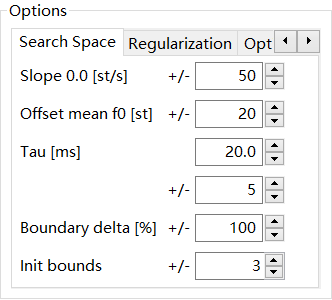
\includegraphics[width=0.3\textwidth]{images/search space.png}
	\caption{Parameters of Search Space}
	\label{ss}
	\end{figure}
	This tab contains all the changeable parameters to determine the search-area of the TO2, as seen in \autoref{ss}. These parameters and their properties are:
	\begin{itemize}
		\item Slope: The maximum slope of each articulatory target, i.e., the slope parameters of the TAM,
		\item Offset mean f0: The maximum offset of each articulatory target,
		\item Tau: The time constant of the critically-damped low-pass filter whose response is f0,
		\item Boundary delta: The boundaries shift factor to adjust the boundaries shift degree. (No boundary shift will be done if set to 0),
		\item Init bounds: The amount of syllable boundaries when using the feature of the initialization of the uniformly boundary positions for the utterance.
	\end{itemize}
	
	\item Regularization
	\begin{figure}[H]
	\centering
	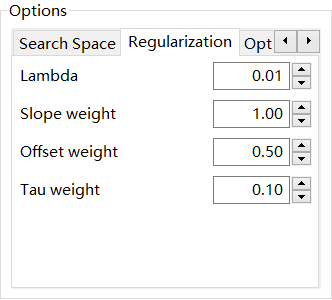
\includegraphics[width=0.3\textwidth]{images/regularization.png}
	\caption{Parameters for Regularization}
	\label{rgl}
	\end{figure}
	In this tab all controllable regularization parameters are listed, as seen in \autoref{rgl}. These parameters and their properties are:
	\begin{itemize}
		\item Lambda: The regularization factor to determine the overall degree of the regularization,
		\item Slope weight, Offset weight, Tau weight: Adjust the degrees of penalization for the different TAM parameters.
	\end{itemize}
	
	\item Optimizer
	\begin{figure}[H]
	\centering
	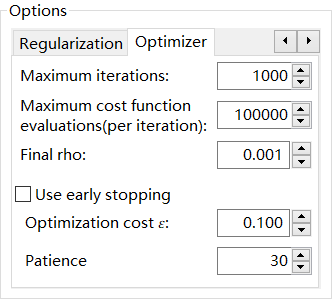
\includegraphics[width=0.3\textwidth]{images/optimizer.png}
	\caption{Hyper-parameters of Optimizer}
	\label{opt}
	\end{figure}
	In this tab all controllable optimization parameters are listed, as seen in \autoref{opt}. These parameters and their properties are:
	
	\begin{itemize}
		\item Maximum iterations: The maximum times of passes of the optimization procedure,
		\item Maximum cost function evaluations (per iteration): The maximal objective function evaluations of each single random iteration,
		\item Final rho: The final trust region radius,
		\item Use early stopping: To terminate the search prematurely as soon as a certain convergence criterion is met,
		\begin{itemize}
			\item Optimization cost $\epsilon$: The optimization factor in terms of the current minimum of TO objective function,
			\item Patience: The threshold of the convergence counter.
		\end{itemize}
	\end{itemize}
\end{itemize}

\subsubsection*{\ding{173} Actions}
As shown in \autoref{act}, the items in Actions are equal to the items in the ``File" menu, i.e.: 
\begin{itemize}
	\item Open File(s): Import the pitch samples of an utterance from a *.PitchTier file, import the target boundaries from *.TextGrid files selecting the ``Position" option. *.PitchTier- and *.TextGrid-files can be imported at the same time by selecting both files in one command window,
	\item Init Bounds: Initialize as many equidistant boundaries as set in ``Init bounds" value in the ``Search Space" options according to the utterance-length,
	\item Optimize Targets: Starts the optimizer with the configured parameters to estimate the pitch contours and boundaries,
	\item Save as...: Export the optimized targets as a table (*.csv file) with pitch target parameters, as a gestural score (*.ges file) to use it in articulatory speech synthesizer like \ding{43} \href{https://www.vocaltractlab.de/index.php?page=start}{VocalTractLab (VTL)}, or as a PitchTier file with the $f_{0}$ samples of the synthesized pitch contour for \ding{43} \href{https://www.fon.hum.uva.nl/praat/}{Praat},
	\item Clear: Clean all data.
\end{itemize}
For more information of file formats, please refer the Appendix \ref{ff}.
\begin{figure}[H]
\centering
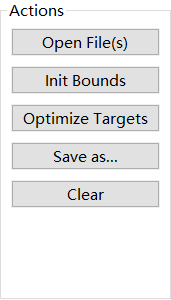
\includegraphics[width=0.2\textwidth]{images/actions.png}
\caption{Actions}
\label{act}
\end{figure}

\subsubsection*{\ding{174} Targets}
Corresponding to the graphs shown in the main window region, the optimized target results are listed in two tables:
\begin{itemize}
	\item ``Target Boundaries" (see \autoref{tb}) presents the values of optimized target boundaries.
	\begin{figure}[H]
	\centering
	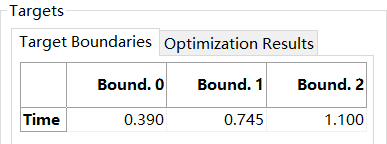
\includegraphics[width=0.35\textwidth]{images/target boundaries.png}
	\caption{Target boundaries}
	\label{tb}
	\end{figure}
	\item ``Optimization Results" (see \autoref{or}) presents the value of optimized pitch contour parameters including slope, offset, tau and the time duration of each target.
	\begin{figure}[H]
	\centering
	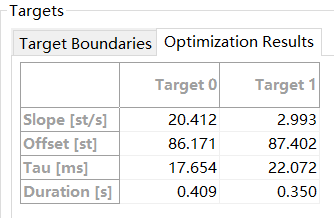
\includegraphics[width=0.35\textwidth]{images/optimization results.png}
	\caption{Optimization results}
	\label{or}
	\end{figure}
\end{itemize}

\section{Command line tool}
To use the software as a command line tool, open the Command Line in Windows or Terminal in Linux and change the directory to the corresponding TargetOptimizer folder, then you can execute the command ``TargetOptimizer -h" to see the following instructions:
\begin{lstlisting}
Usage: TargetOptimizer <PitchTier-file> <LOG-name> { <options> | <arg> }
Options:
 -h                           Display this help message.
Additional Parameter Options:
 --b-range <arg>              Specify search space for offset parameter.
 --b-weight <arg>             Specify regularization weight for offset parameter.
 --boundaryDelta <arg>        Specify boundary delta.
 --epsilon <arg>              Specify the epsilon for early stopping
 --initBounds <arg>           Specify how many bounds should be initialized.
 --lambda <arg>               Specify regularization parameter.
 --log                        Outputs f0, targets, boundaries, etc. to a single text file.
 --m-range <arg>              Specify search space for slope parameter.
 --m-weight <arg>             Specify regularization weight for slope parameter.
 --maxCostEvaluations <arg>   Specify maximum number of costfunction evaluations.
 --maxIterations <arg>        Specify maximum number of optimizer iterations.
 --patience <arg>             Specify the patience for early stopping
 --rhoEnd <arg>               Specify the rho_end parameter.
 --t-range <arg>              Specify search space for time constant parameter.
 --t-weight <arg>             Specify regularization weight for time constant parameter.
 --tg <arg>                   Specify a TextGrid file.
 --useEarlyStopping           Stop the search early if fmin-ftmp < epsilon for times (x=patience).
 --utterance <arg>            Name of the utterance to optimize.
Output Options:
 -c                           Choose for csv table file.
 -g                           Choose for VTL gesture file.
 -p                           Choose for PitchTier file. 
\end{lstlisting}
For a (non-advanced) pitch contour extraction for the german word ``Buch" the corresponding command would be
\begin{lstlisting}
TargetOptimizer Buch.PitchTier --tg Buch.TextGrid,
\end{lstlisting}
whereas an analysis with custom paramaters could look like
\begin{lstlisting}
TargetOptimizer Buch.PitchTier --tg Buch.TextGrid --lambda 0.2 --patience 40
\end{lstlisting}
\chapter{TO2 as part of natural articulatory speech synthesis}\label{chap:synthesis}

One of TO2's main purposes is to act as an interface between an audio analysis program, mainly Praat (\ding{43} \href{https://www.fon.hum.uva.nl/praat/download_win.html}{Download}), and an articulatory speech synthesizer, namely VocalTractLab (VTL) (\ding{43} \href{https://www.vocaltractlab.de/index.php?page=vocaltractlab-download}{Download}), to obtain optimized pitch-curves for the synthesis of more natural speech. \autoref{flow} illustrates this workflow and shows which interface information is required and produced at each step. The input data for the TO2 are a TextGrid file with syllable boundaries (which is optional since v2.0) and a PitchTier file with the $f_{0}$ samples to be reproduced by TAM. Both files are created with the software Praat (\ding{43} \href{https://www.fon.hum.uva.nl/praat/download_win.html}{Download}) from the audio file of the original utterance. The parameters of TO2 can be configured by using the GUI or the command line tool. The optimized results from TO2 can be saved as a gestural score (*.ges file) which can then be used inside of VTL.

\begin{figure}[H]
\centering
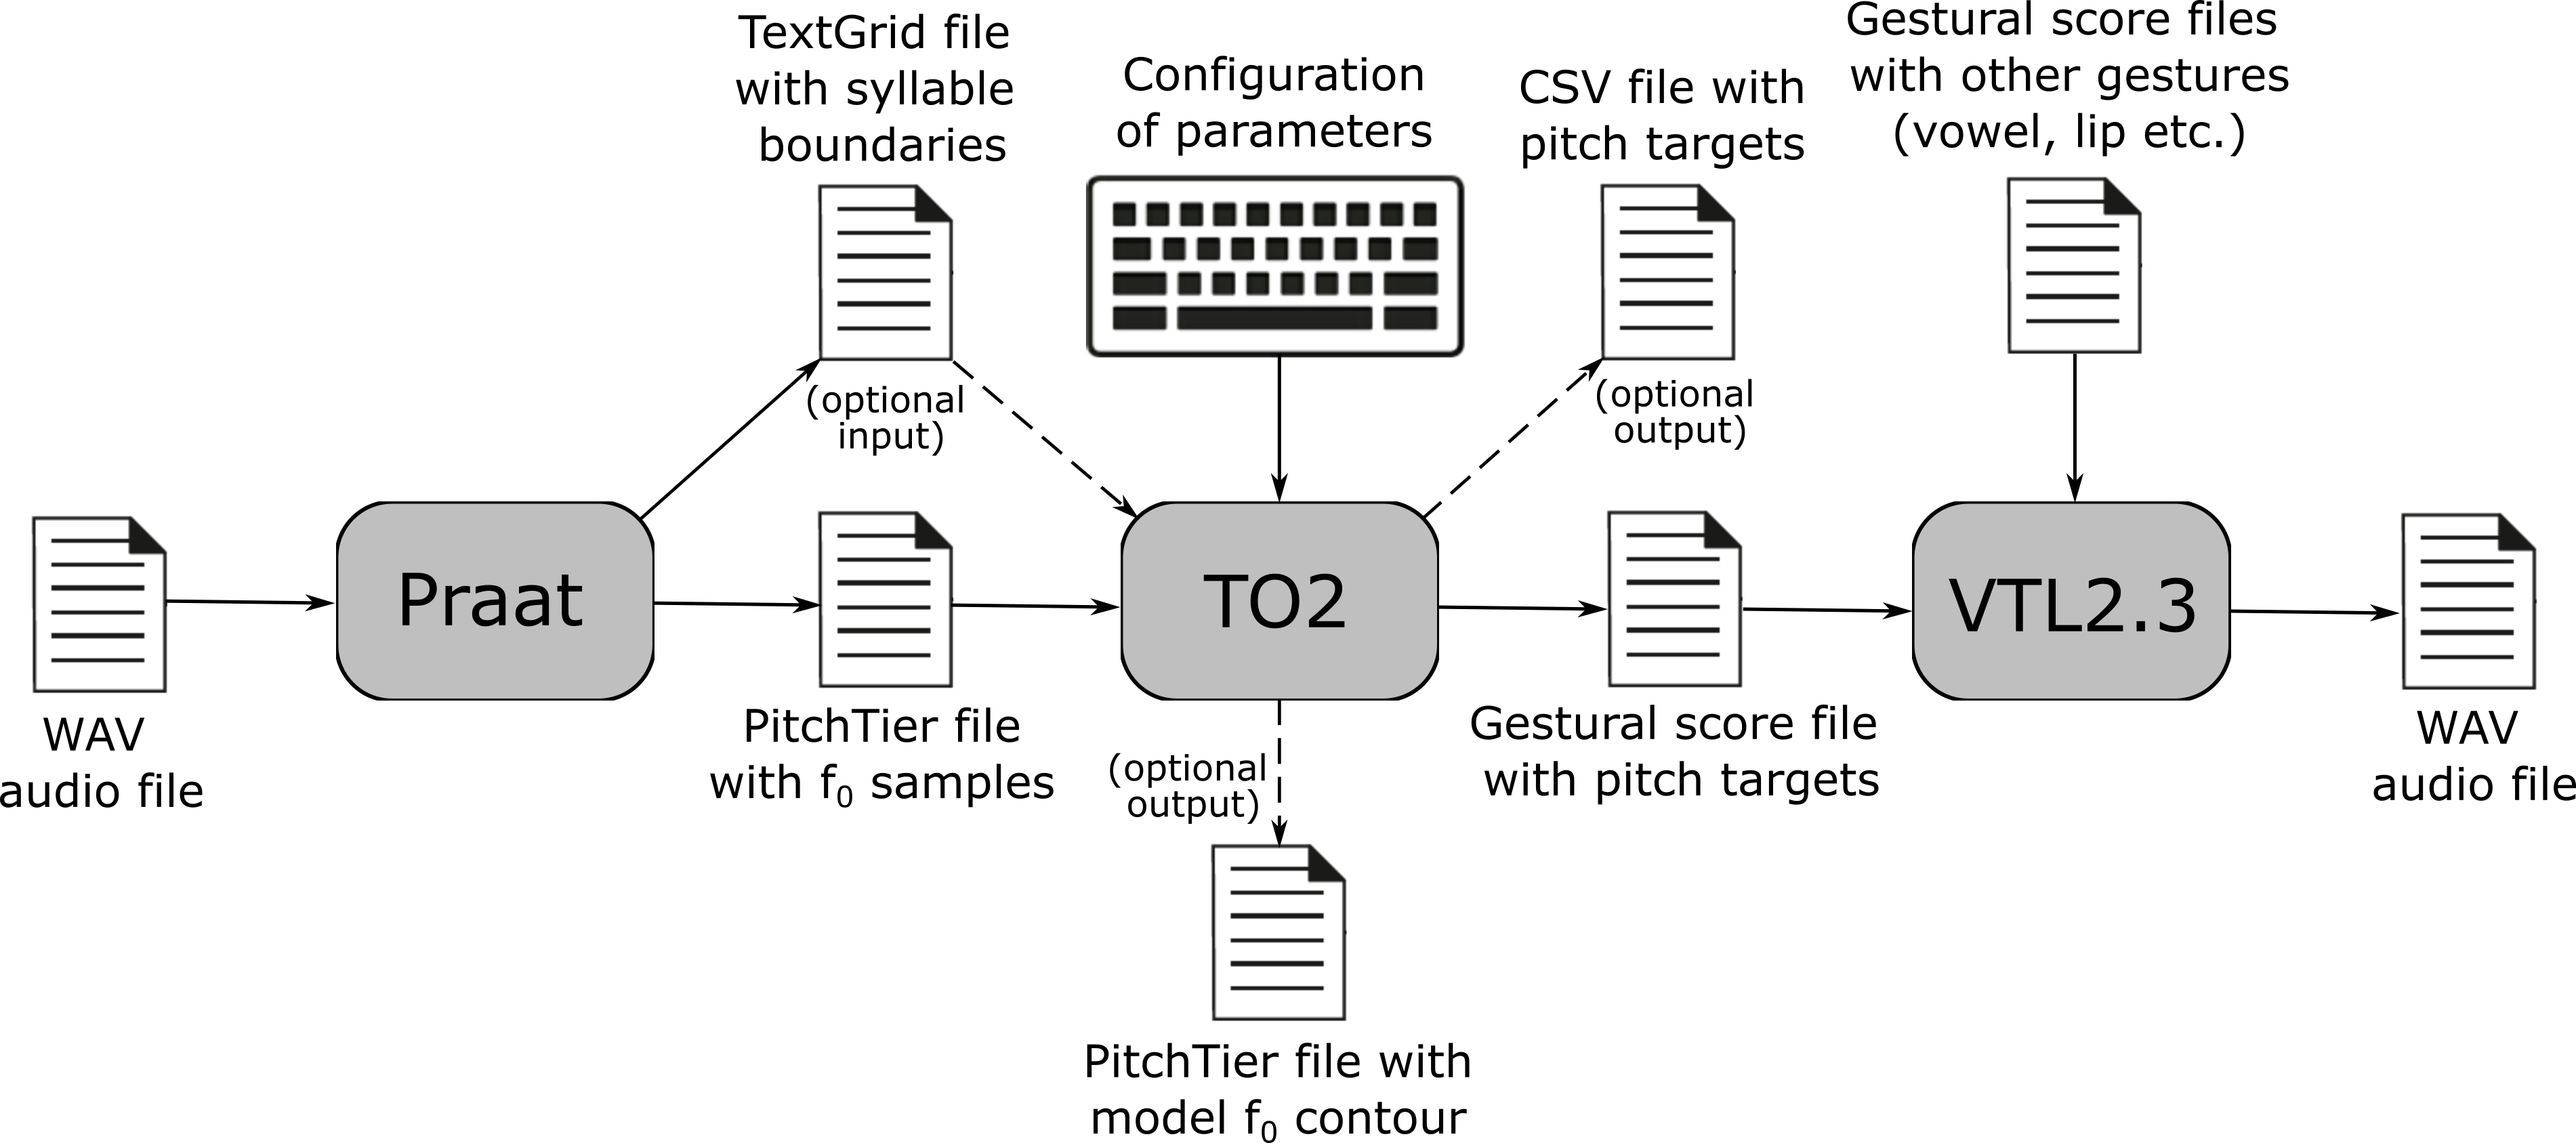
\includegraphics[width=0.9\textwidth]{images/flow.png}
\caption{
Articulatory speech synthesis pipeline}
\label{flow}
\end{figure}

In the following sections this workflow is shown step by step for the german word ``Ästhetik".

\section{Praat}

\begin{figure}[H]
\centering
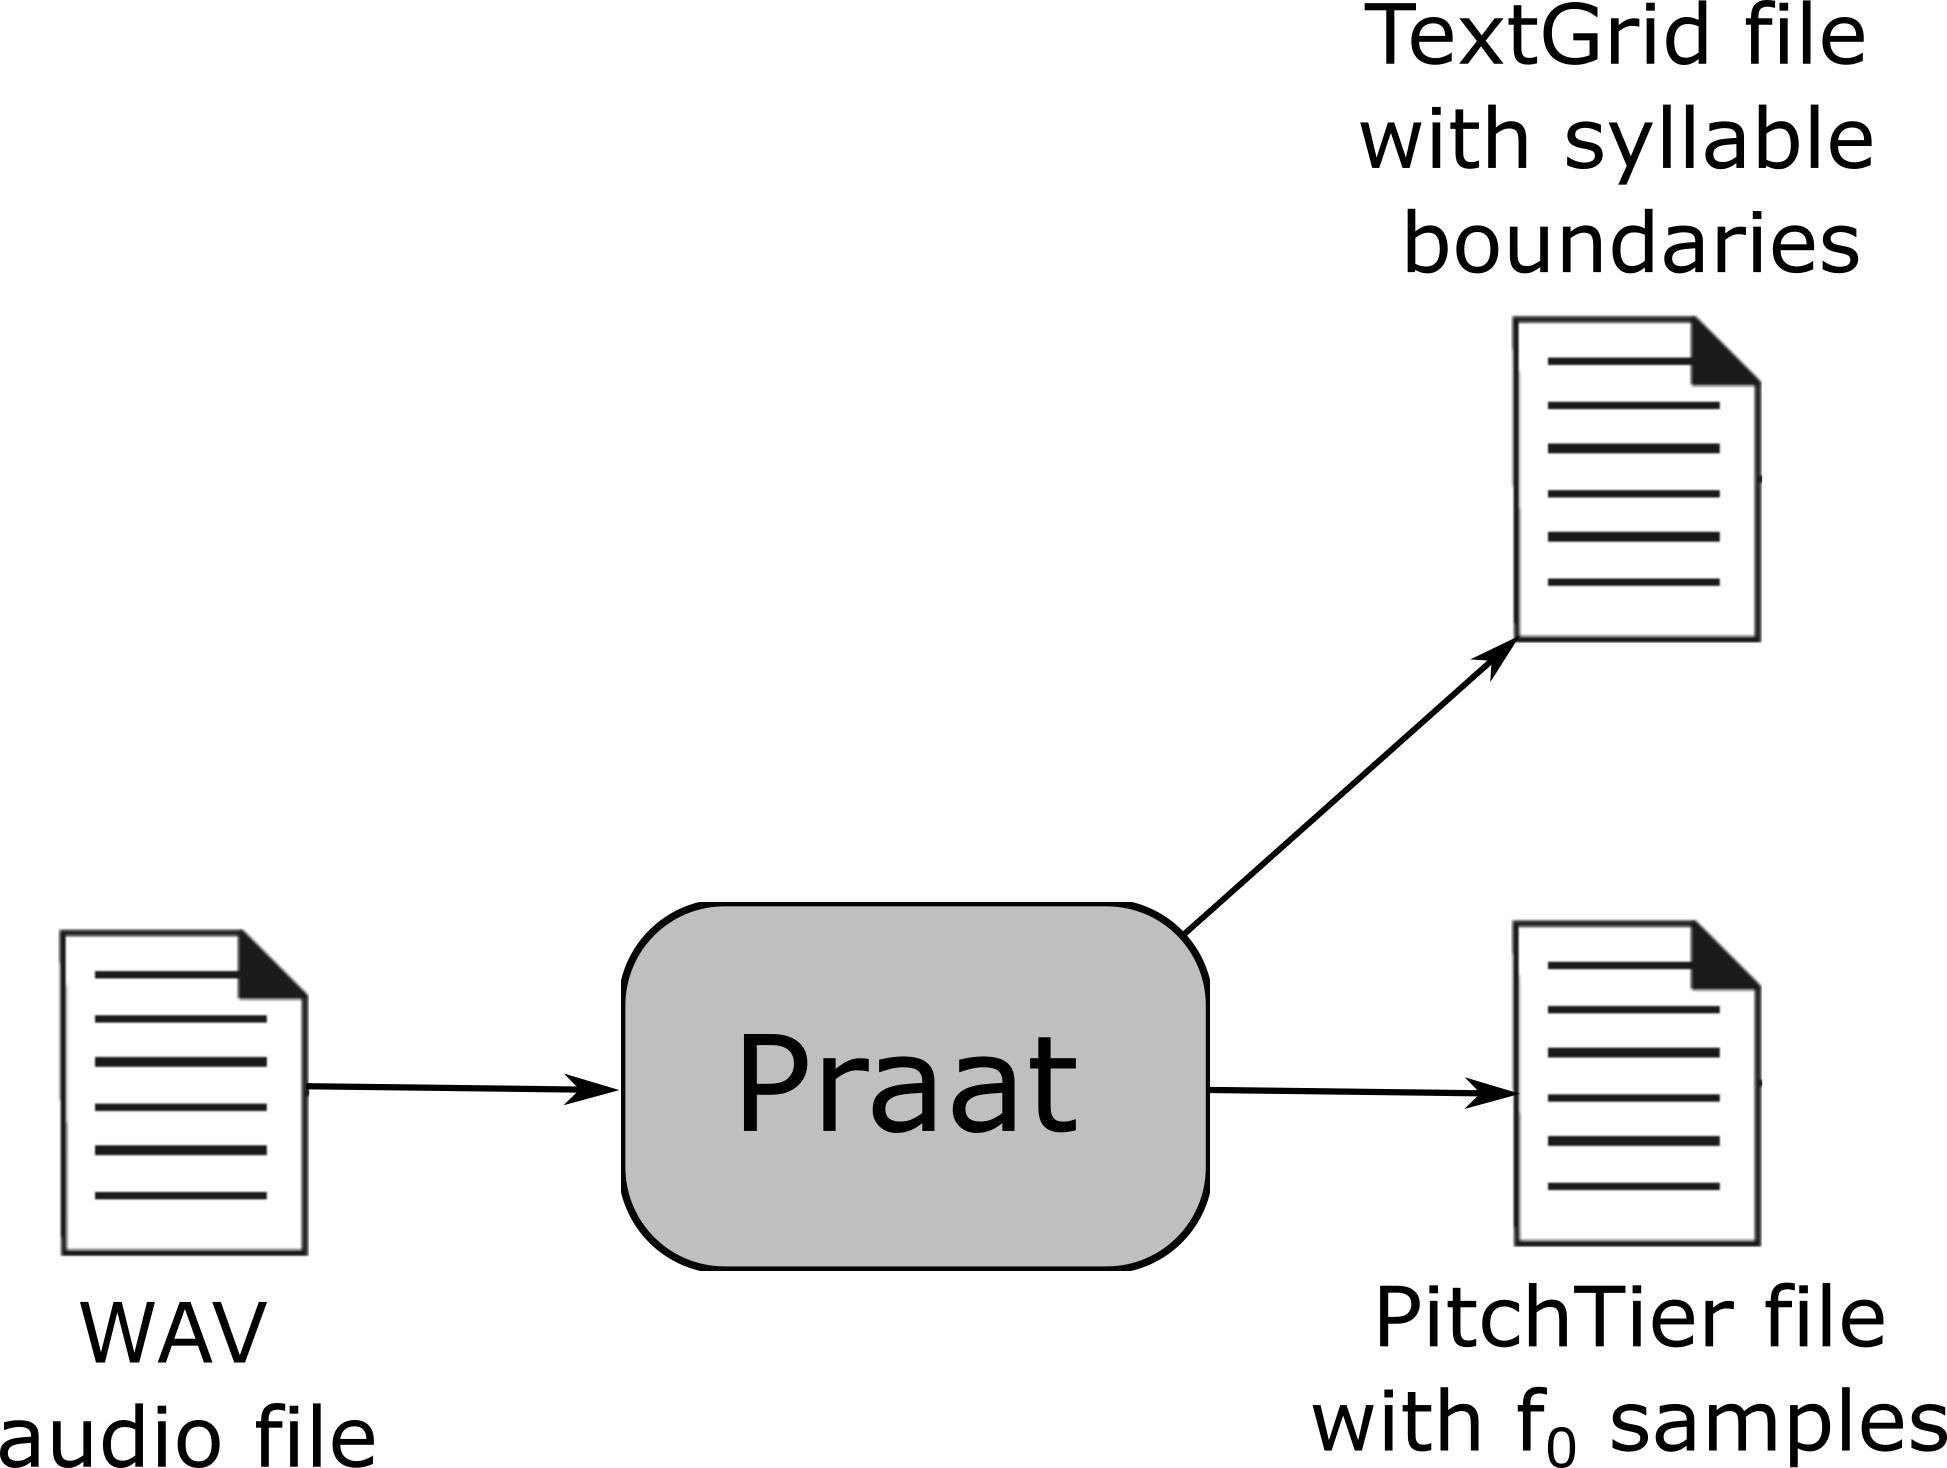
\includegraphics[width=0.4\textwidth]{images/3_11.png}
\caption{Input and outputs of Praat}
\label{3_11}
\end{figure}

Praat is used to obtain pitch frequencies and segment boundaries from a spoken utterance. Those information can be exported as a TextGrid file for the segment boundaries or as a PitchTier file for the pitch.\\
Therefore the utterance is imported into Praat and segmented. Segmentation takes place on syllable level and not phonetically. The pitch analysed is then extracted and those information exported. 

\begin{figure}[H]
\centering
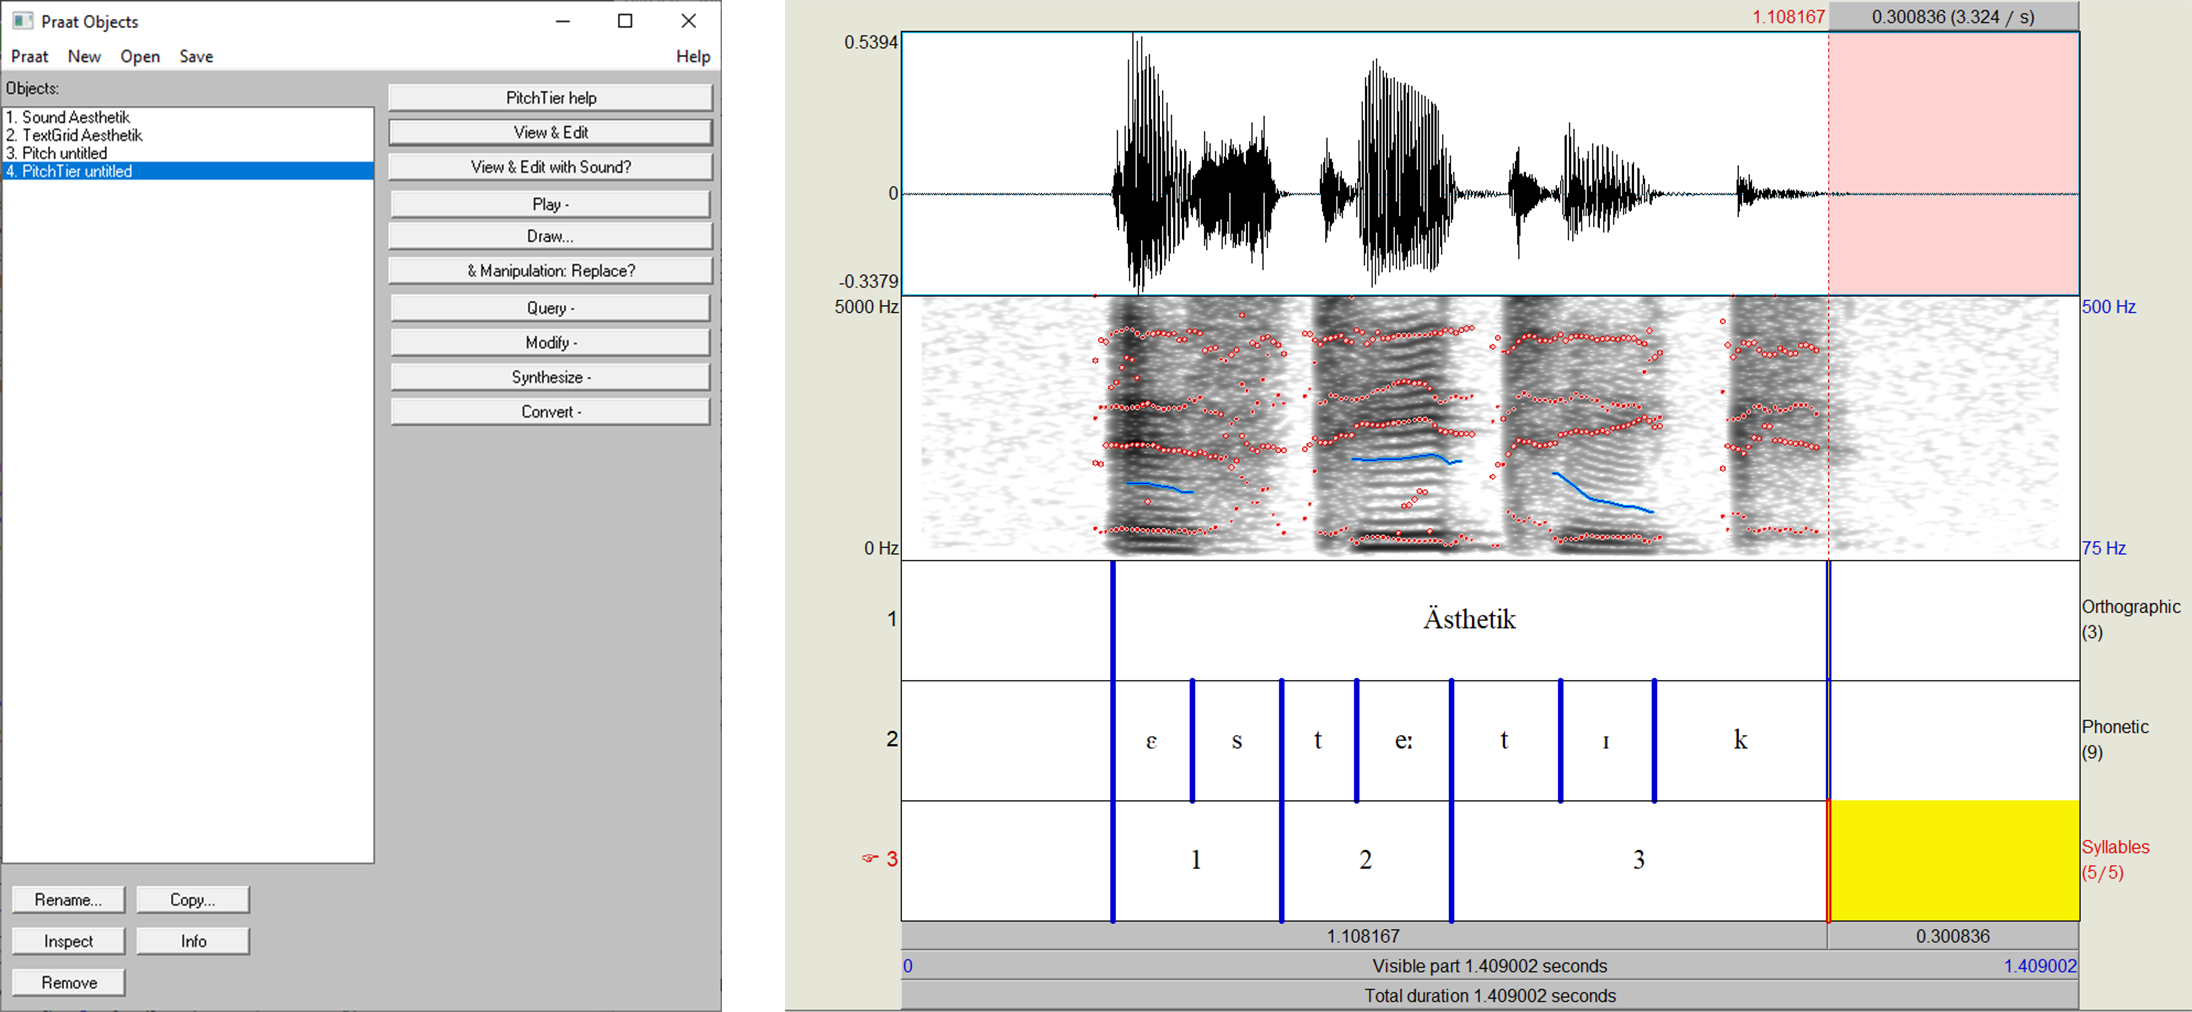
\includegraphics[width=0.9\textwidth]{images/3_12.png}
\caption{Praat GUIs: a) Objects Window, b) Editor Window}
\label{3_12}
\end{figure}

This procedure can be done with the following steps:

\begin{enumerate}
	\item In the Objects Window (see \autoref{3_12} a) ) import the sound file you want to analyse via ``Open" $\to$ ``Read from file..." or create a new record via ``New" $\to$ ``Record mono Sound...". A new Sound Object appears in the Objects Window list. 
	\item Select this Sound Object and use the function ``Annotate" $\to$ ``To TextGrid..." $\to$ $<$insert the tier names e.g. [Orthographic Phonetic Position]$>$ to obtain a new empty TextGrid which appears in the Objects Window list.
	\item Select both the Sound Object and the TextGrid Object and use the function View \& Edit to open both in the Editor Window. In this window you can segment and label the utterance in the tiers as you need it. Every change will be saved automatically in the TextGrid Object.
	\item In the Editor Window click on the menu ``Pitch" $\to$ ``Extract visible Pitch contour" to extract the automatically analysed pitch frequencies. A new Pitch Object appears in the Objects Window.
	\item Select the Pitch Object in the Object Window and use the function ``Convert" $\to$ ``Down to PitchTier". This creates a PitchTier Object. 
	\item To export the pitch frequencies in the PitchTier Object click on the menu `Save" $\to$ ``Save as PitchTier spreadsheet file..." and save the PitchTier file to your desired folder. 
	\item To export the target boundaries in the TextGrid Object click on the menu `Save" $\to$ ``Save as text file..." and save the TextGrid file to your desired folder. Be aware that the TO2 needs the TextGrid to be ecnoded in UTF-8 format. If you have special letters in the TextGrid file Praat is not able to convert this file to UTF-8. Please use another program to convert this file, e.g. Notepad++., before importing it in TO2.
\end{enumerate}

\section{TO2}

\begin{figure}[H]
\centering
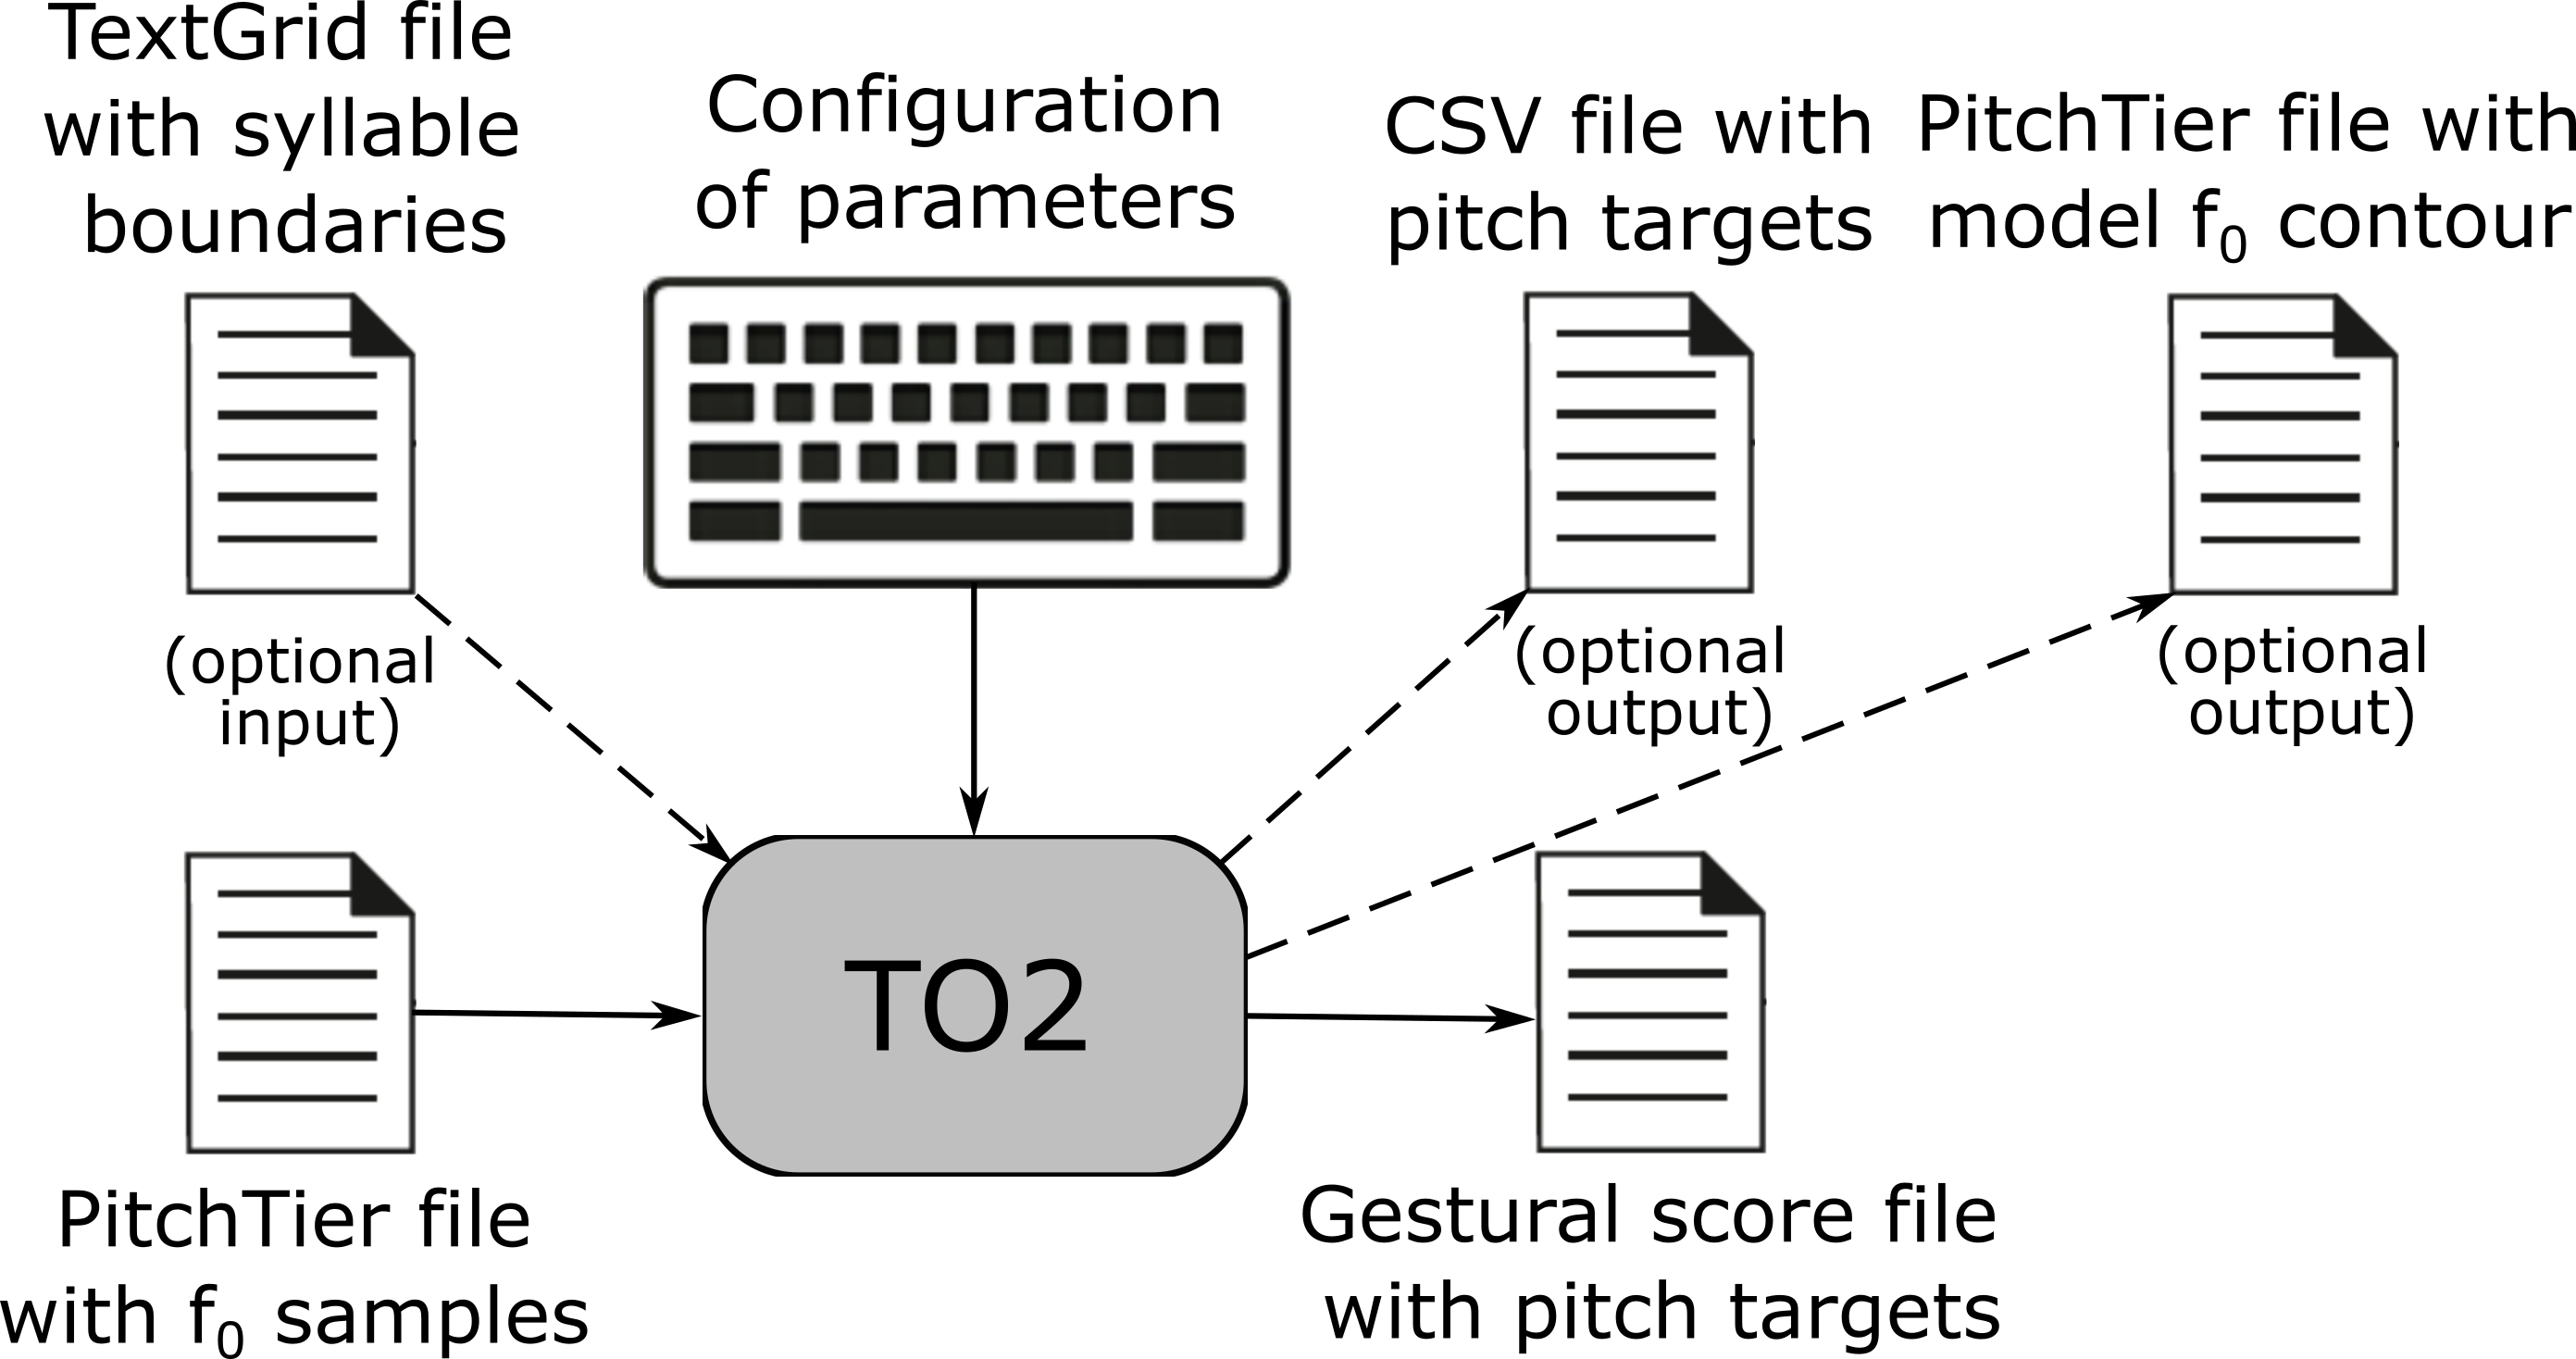
\includegraphics[width=0.4\textwidth]{images/3_21.png}
\caption{Input and outputs of TO2}
\label{3_21}
\end{figure}

The TO2 uses the PitchTier file and (not necessarily) the TextGrid file to perform a target optimization and obtain the pitch targets.

\begin{figure}[H]
\centering
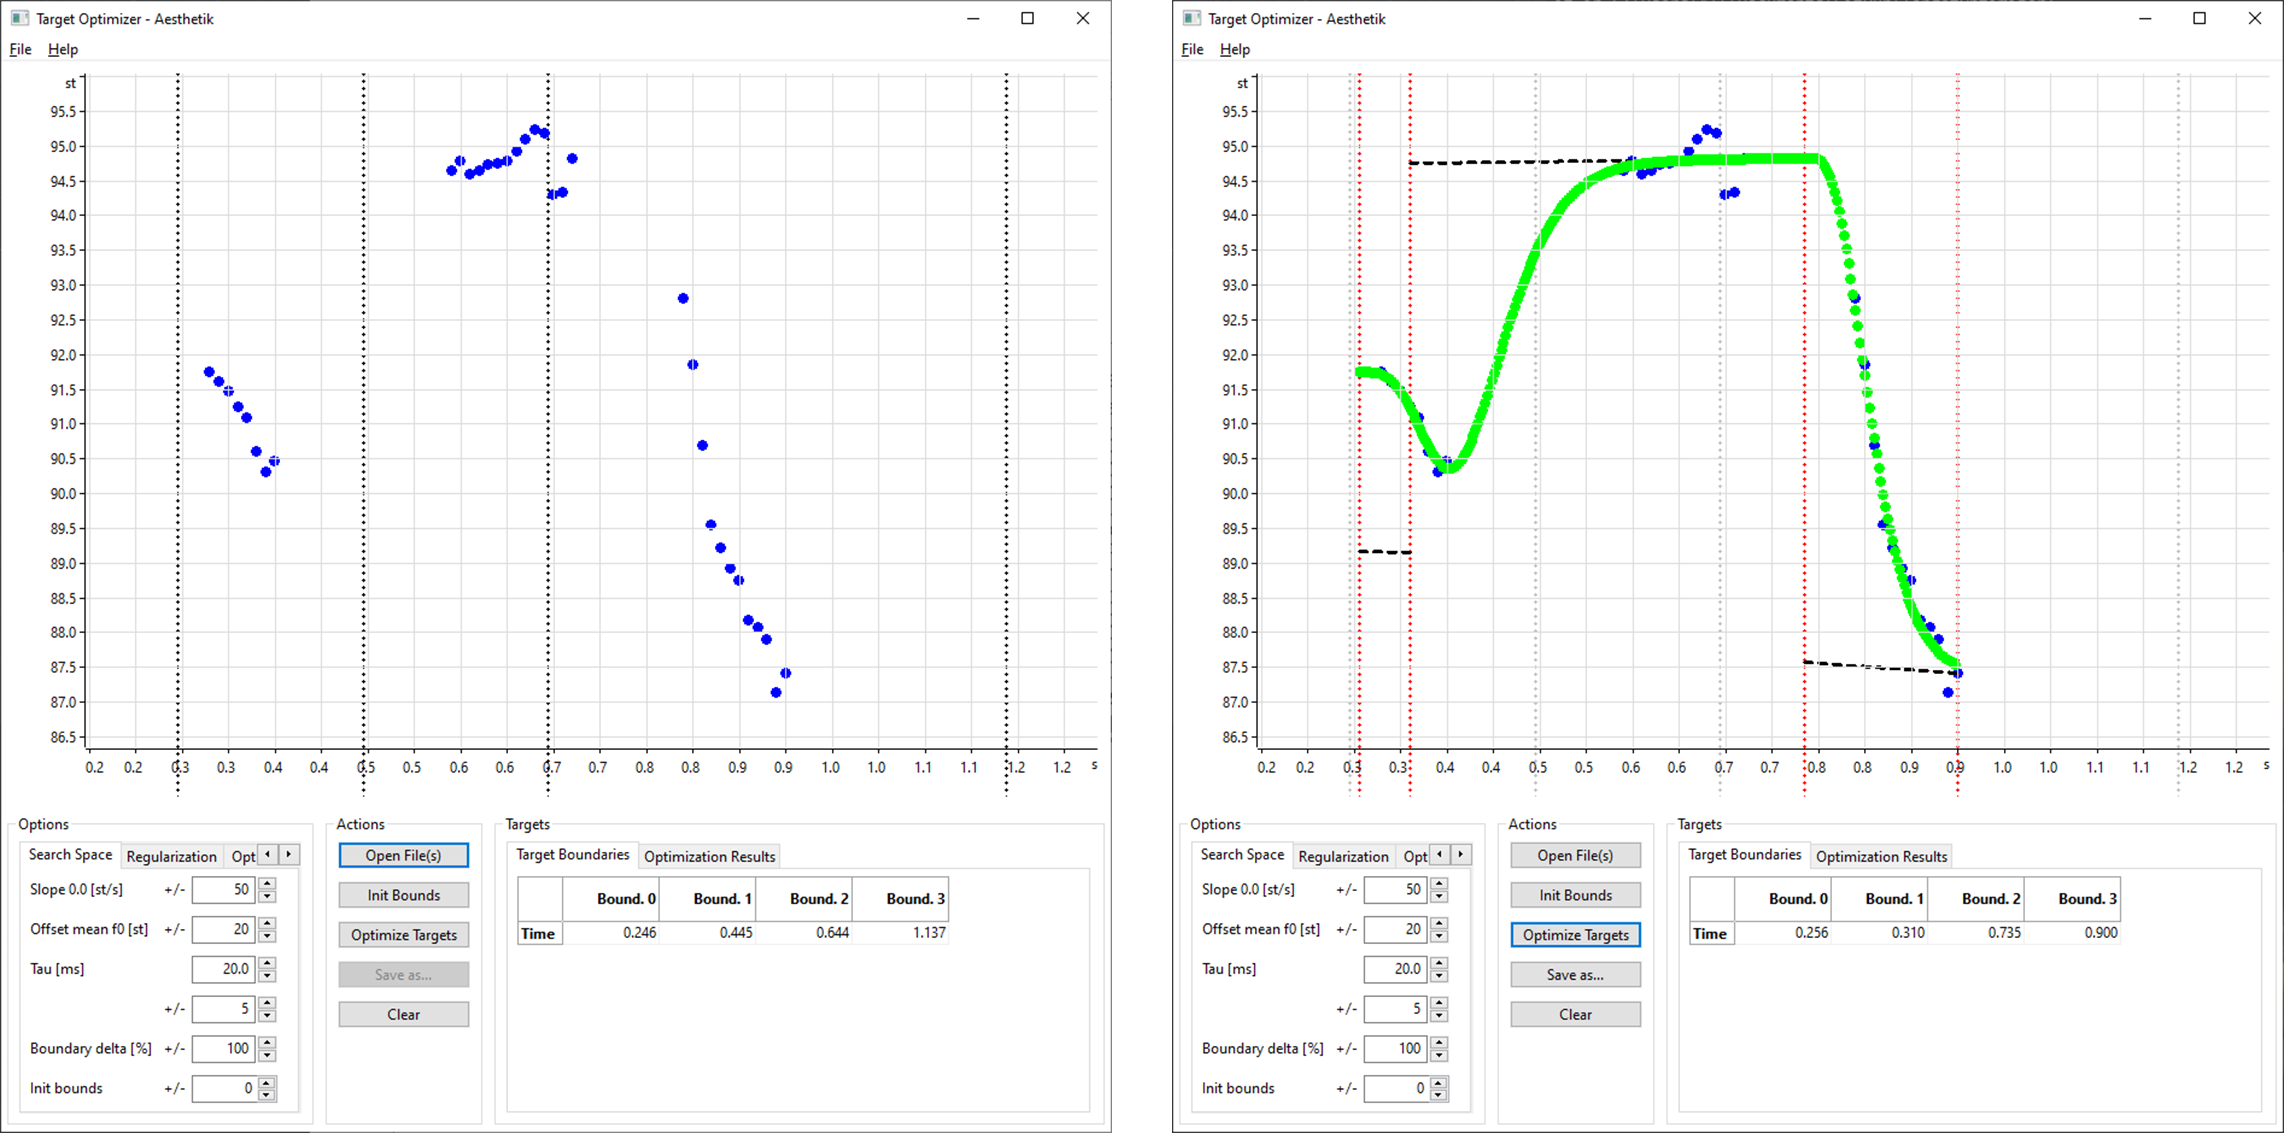
\includegraphics[width=0.9\textwidth]{images/3_22.png}
\caption{TO2 GUI: a) with imported PitchTier and TextGrid and b) with optimized pitch contour}
\label{3_22}
\end{figure}

Following steps are necessary to successfully estimate targets for an utterance:
\begin{enumerate}
	\item Open the pitch contour from the Praat PitchTier file.
	\item Input the corresponding boundaries. This can be performed by opening a Praat TextGrid file (UTF-8 encoded) or by using the equidistant boundary function of the TO2. To set equidistant boundaries type the amount of desired boundaries into ``Init bounds" option and click the ``Init Bounds" button. Afterwards the graph looks similar to Fig. \ref{3_22}a).
	\item Carefully think about the parameters you want to change (the default values are generally well suited).
	\item To perform the Target Approximation click the``Optimize" button. After the calculation the interpolated pitch contour is visible in the graph (see \autoref{3_22}b) ).
	\item Export the results as a *.ges file for VTL. 
\end{enumerate}

\section{VTL2.3}

\begin{figure}[H]
\centering
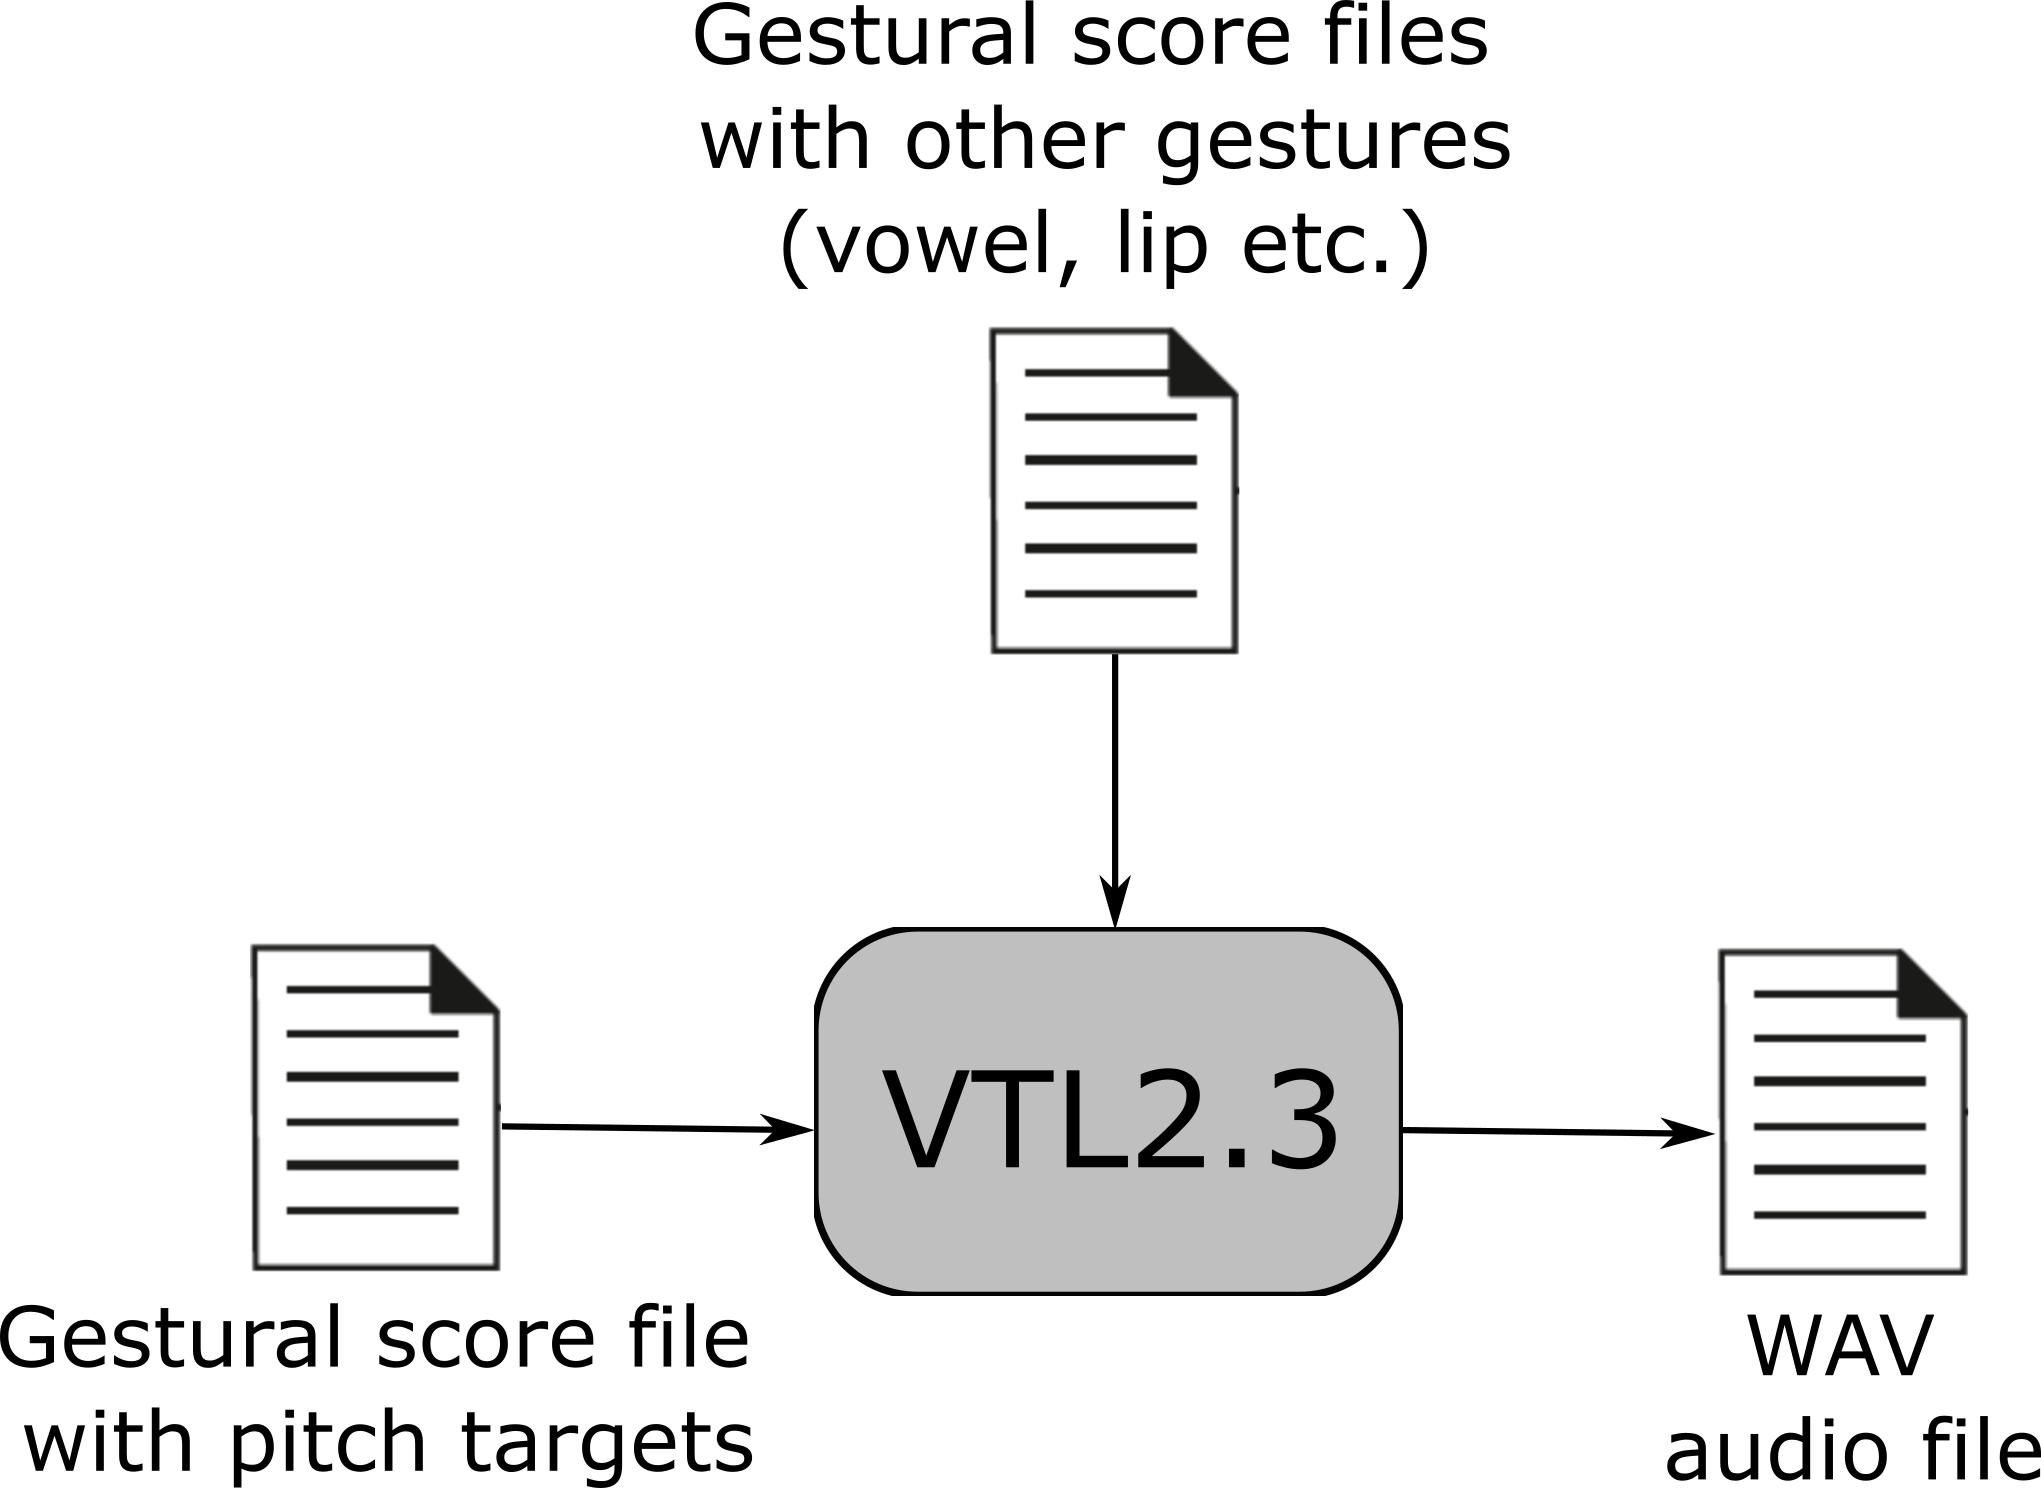
\includegraphics[width=0.4\textwidth]{images/3_31.png}
\caption{Input and outputs of VTL}
\label{3_31}
\end{figure}

The optimized pitch contour can now be used for articular speech synthesis in VTL. This can be done as follows:
\begin{enumerate}
	\item To import the pitch-contour information press ``File" $\to$ ``Load gestural score" and select the desired *.ges file.
	\item Click the ``Gestural score" in the toolbar to go to the gestural score page. In the gestural line ``F0 gestures" the information is now loaded and can be used for the synthesis.
\end{enumerate}

\appendix
\chapter{File formats}\label{ff}
\begin{itemize}
    \item \textbf{PitchTier file (*.PitchTier)}\\
    PitchTier is one of the types of objects in Praat that represents a time-stamped pitch contour, i.e., it contains a number of (time, pitch) points, without voiced/unvoiced information. The PitchTier objects are used for two purposes: for manipulating the pitch curve of an existing sound and for synthesizing a new sound.\\
    For more information about PitchTier, please refer to \ding{43} \href{https://www.fon.hum.uva.nl/praat/manual/PitchTier.html}{PitchTier}.

    \item \textbf{TextGrid file (*.TextGrid)}\\
    TextGrid is one of the types of objects in Praat, which is used for annotation (segmentation and labelling). A TextGrid object includes two kinds of tiers: an interval tier is a connected sequence of labeled intervals, with boundaries in between; A point tier is a sequence of labeled points. It is important that the TextGrid file is encoded in UTF-8.\\
    For more information about TextGrid, please refer to \ding{43} \href{https://www.fon.hum.uva.nl/praat/manual/TextGrid_file_formats.html}{TextGrid}.

    \item \textbf{Gestural score file (*.ges)}\\
    A gestural score file is an XML file that defines a gestural score. The gestural score is an organized pattern of articulatory gestures for the realization of an utterance. The root element of the file is \textsl{gestural\_score}. There are eight tiers of gestures in a gestural score, each of which is represented by one \textsl{gesture\_sequence} element. Each gesture sequence comprises a set of successive gestures of the same type. The start time of a gesture is implicitly given by the sum of durations of the previous gestures of the sequence.\\
    For more information about gestural score, please refer to \ding{43} \href{https://www.vocaltractlab.de/download-vocaltractlab/VTL2.3-manual.pdf}{VTL2.3-manual}.
\end{itemize}
\chapter{Major Changes from version 1.0 to 2.0}
\begin{itemize}
	\item I/O routines are enhanced which makes the software much more flexible and robust against undefined behavior induced by wrong file types.
	\item We tuned all free parameters on a test corpus to find optimal default values.
	\item We developed a new GUI based on the wxWidgets C++ library.
	\item We have extended a command line functionality.
	\item The position of target boundaries is now a fully optimizable parameter, which can be freely moved up to 100\% of syllable long. 
	\item The amount of bounds can be manually set according to the utterance without loading the corresponding TextGrid file.
	\item The time constant $\tau$ can be manually adjusted.
	\item Optimizer options such as: restrain the maximal iteration and cost function, use the early-stopping etc. are added to avoid over-fitting and reduce the computational overload.
\end{itemize}
\chapter{Credits}
\section{Developers of TargetOptimizer 1.0}
TargetOptimizer 1.0 was developed by Patrick Schmager and has been released under supervision of Peter Birkholz. TO1 has served as basis for the developement of TO2, which has been described in preceding chapters.

\section{Developers of TargetOptimizer 2.0}
TargetOptimizer 2.0 was deveveloped by Paul Konstantin Krug, Simon Stone (né Preuß) and Alexander Wilbrandt. It has been released under supervision of Peter Birkholz.

\section{Documentation}
This manual has been drafted by Arne-Lukas Fietkau and Yifei Li.

\section{Supervision}
The coding process and the final release have been supervised by Peter Birkholz.

\chapter*{Acknowledgments}

\bibliography{References}
\bibliographystyle{unsrt}

\end{document}
